\documentclass[english,a4paper,12pt,oneside]{article}


%\includeonly{lab4}

%Drafting options
%uncomment for double spacing
%\doublespacing 

% \usepackage{acronym}
\usepackage{times}
\usepackage{setspace} 
\usepackage{amsmath}    % need for subequations
\usepackage{graphicx}   % need for figures
%\usepackage{picture}
% \usepackage{wrapfig}
\usepackage{graphics}
 \graphicspath{{./}{../plot/}{../data/}}
 \usepackage{epstopdf}
\usepackage{color}
\usepackage{listings}
\lstset{language=matlab,
	basicstyle=\ttfamily\footnotesize,
	breaklines=true,
%    basicstyle=\ttfamily,
    keywordstyle=\color{blue}\ttfamily,
    stringstyle=\color{red}\ttfamily,
    commentstyle=\color{green}\ttfamily,
%    morecomment=[l][\color{magenta}]{\#}
}
\usepackage{verbatim}   % useful for program listings
\usepackage{color}      % use if color is used in text
\usepackage{subfigure}  % use for side-by-side figures
\usepackage{varioref}
\usepackage{anysize}
\usepackage{natbib}
\usepackage{fancyhdr}
% \usepackage{units}
\usepackage{longtable}
%\usepackage{bbding}
%\usepackage{aeguill}
\usepackage[hyphens]{url}
\usepackage{hyperref}

\setlength{\parskip}{8pt plus 2pt minus 2pt}
\setlength{\parindent}{0pt}

\marginsize{2cm}{2cm}{2cm}{2cm}
\fancypagestyle{plain}{%
  \fancyhf{}%
  \renewcommand{\headrulewidth}{0pt}%
  \renewcommand{\footrulewidth}{0pt}%
}

\pagestyle{fancy}
%\renewcommand{\sectionmark}[1]{\markright{\thesection.\ #1}}

\renewcommand{\sectionmark}[1]{\markright{#1}{}}
\renewcommand{\subsectionmark}[1]{\markright{#1}{}}
\renewcommand{\subsubsectionmark}[1]{\markright{#1}{}}

%\renewcommand{\quote}[1]{\textit{\begin{quote}#1\end{quote}}}
\newcommand{\bold}[1]{\emph{\textbf{#1}}}

\newcommand{\varentry}[1]{{\guillemotleft}\emph{#1}{\guillemotright}}
\newcommand{\code}[1]{{\tt #1}}

\headheight 10mm


\rhead{22/10/2018}
\chead{}
\lhead{ICP3038 --- Computer Vision}
\rfoot{}
\cfoot{- \thepage  \,\,-}
\lfoot{}

\renewcommand{\headrulewidth}{0.4pt}
\renewcommand{\footrulewidth}{0.4pt} 



\begin{document}
% !TEX root = ./ICP3038_Lab_03.tex

\section*{Laboratory 5: How to compare apply a convolution filter on 1D arrays}

%This is a typical script that you will be working with at each
%laboratory session. To work with these scripts efficiently, follow the
%guidelines below.
%\begin{enumerate}
%  \item The script is not a step-by-step tutorial. It introduces the
%    problem but it is your task to solve it.
%
%  \item If you get stuck, make sure that you read \emph{Help} section
%    at the end of the document.
%
%  \item If you still have problems, ask the lecturer, demonstrator or
%    fellow students for help.
%
%  \item Try to do as much work as possible in the class, where it is
%    easier to get help.
%    
%  \item If you need help when working at home, use the Blackboard
%    discussion board.
%    
%  \item Finish all assignments at least a week before the deadline. If you get
%    stuck, you will still have one week to ask for help.
%\end{enumerate}

The aim of today's lab is to:
\begin{itemize}
	\item Extend last week's implementation to support 1-D convolution.
	\item Add two low-pass filters.
	\item Add a high-pass filter.
	\item Compute the gradient magnitude.
	\item Implement a median filter.
%	\item Compare two arrays using \verb+operator==+ and \verb+operator!=+.
\end{itemize}

Note that today you work using 1-D arrays. In Assignment~2, you have to do the same in 2-D with images. It is straightforward to extend the implementation to 2-D. 

\section*{Task 0: Setting up}

%Same as usual, we will use CMake to make our lives easier. 
%In the lecture, you saw yesterday that it can be extremely complicated to use the IDE to maintain the project files, etc. particularly if students use Windows, Mac, or Linux. 
%There is a ZIP file on Blackboard with 4 (almost) empty C++ source files. There is also a `CMakeLists.txt' file. 
%It is a good practice to organise your source code using directories, etc. Do not compile code in the same directory as your source code. It can get messy... 
%Extract the ZIP file, and set up the compilation environment using \verb+cmake+. 
%In the GUI, the source directory corresponds to the direction in which `CMakeLists.txt' is. 
%The binary directory is where the code will be compiled. Often, we call this directory `bin'. 
%Once the paths are set, press `Configure'. 
%The first time you run the configuration tool, you have to select a generator.
%If you want to use MSVC++ in the lab, make sure to use \emph{Visual Studio 14 2015 Win64}. 
%For Mac OS X, you may want to use the Xcode generator. 
%For Linux, you may choose Makefile. 
%Once the configuration step is over, press `Generate'. 
%The project files are now ready in the `bin' directory. 
%You can compile the code using the preferred IDE.
There is not so much to do this week. We will use the project from last week and modify \verb+MyVector.h+ to add new method definitions, \verb+MyVector.cpp+ to implement them, and \verb+test_my_vector+ to test them.

I added two new methods to save data in ASCII files, so that we can plot it in Matlab. 
See files on Blackboard.


\section*{Task 1: convolve()}

\verb+m+ is the input vector, and \verb+g+ is the kernel (sliding window). 
\verb+m+  has length \verb+N+ and \verb+g+ has length \verb+L+.
\verb+m'+ is the result of the convolution of \verb+m+ by \verb+g+: %$(m'(i) = (m * g)(i)$.

$$
m'(i) = (m * g)(i) = \sum^{k < L}_{k=0} m(i - L \setminus 2 + k) \times g(k)
$$
with $\setminus$ the symbol of integer division ($3 \setminus 2 = 1$).

Add a new method \verb+convolve+ that returns a new instance of \verb+MyVector+ and takes the kernel as parameter (e.g. as an array of 3 floating point numbers):

\verb+MyVector convolve(const float* apKernel) const+. Two nested (for) loops are required to implement the convolution in 1-D. One is used to process all the samples of the vector; one for all the coefficients of the kernel. 

Let us consider the pseudocode below where
\verb+m'+ is the results of the convolution of \verb+m+ by \verb+g+:





\begin{verbatim}
Create a new vector m' of size N, with N the size of m
Initialise all the elements of m' to 0
for all the samples i in the vector m
do
     for all the coefficients k in the kernel g, with 0 <= k < L
     do
         m'[i] += m[i - L \ 2 + k] * g[k]
     done
 done
\end{verbatim}

The first and last samples of \verb+m+ are special cases:
\begin{enumerate}
\item \verb+m[-1]+ is not defined.
\item \verb+m[N]+ is not defined.
\end{enumerate}

The two main methods to deal with this problem are called 0 padding and clamping. 
\begin{enumerate}
\item 0 padding is easy to implement: \verb+m[i]+ is equivalent to 0 if \verb+i+ is less than zero or equal to or greater than  \verb+N+. 
\item Clamping is more elegant and quite easy to implement, so it is recommended over zero padding. \verb+m[i]+ is equivalent to \verb+m[0]+ if \verb+i+ is negative, and it is equivalent to \verb+m[N-1]+ if \verb+i+ is equal to or greater than  \verb+N+. 
\end{enumerate}



\section*{Task 2: Preset filters}

Note that you have to use a temporary variable to store the convolution kernel, 

e.g. 
\verb+float p_kernel[] = {1.0f / 3.0f, 1.0f / 3.0f, 1.0f / 3.0f};+.



\begin{enumerate}
\item Mean filter: The kernel is $\left[1.0/3.0~~~1.0/3.0~~~1.0/3.0\right]$.

Add a new method called \verb+MyVector meanFilter() const+. 
In it, just return the result of the method \verb+convolve+ with 
\verb+{1.0f/3.0f, 1.0f/3.0f, 1.0f/3.0f}+ as parameter.

\item Gaussian filter: The kernel is $\left[1/4~~~2/4~~~1/4\right]$. 

Add a new method called \verb+MyVector gaussianFilter() const+. 
In it, just return the result of the method \verb+convolve+ with \verb+{1.0f/4.0f, 2.0f/4.0f, 1.0f/4.0f}+ as parameter.

\item Derivative filter: The kernel is $\left[1~~~0~~~-1\right]$. 

Add a new method called \verb+MyVector derivativeFilter() const+. 
In it, just return the result of the method \verb+convolve+ with \verb+{1.0f, 0.0f, -1.0f}+ as parameter.

\end{enumerate}

\section*{Task 3: Gradient magnitude}

We will add two methods:
\begin{enumerate}
\item \verb+MyVector abs() const+: 
It returns a new vector \verb+m'+ whose size is the same as the input vector \verb+m+, so that \verb+m'[i] = abs(m[i])+. Note that the \verb+abs+ function is defined in the header file \verb+<cmath>+ (no dot h).



\item \verb+MyVector gradientMagnitude() const+: 
The gradient magnitude is the result of the derivative filter without taking into account the sign (+/-). This is why the \verb+abs+ method is used in addition to the \verb+derivativeFilter+ method.


\end{enumerate}


\section*{Task 4: Median filter}


The median filter is not a convolution. Let us consider the case when \verb+m'+ is the result of the median filter on \verb+m+.  Every sample \verb+i+ in \verb+m'+ corresponds to the median value of the neighbours of \verb+m[i]+ within a given radius.
Again, two nested (for) loops are required in the 1-D case. One is used to process all the samples of the vector; one for all the neighbourgs. 

Let us consider the pseudocode below. 
\begin{verbatim}
Create a new vector m' of size N, with N the size of m
Initialise all the elements of m' to 0
for all the samples i in the vector m
do
     create a new STL vector temp
     for all the neighbours n in the radius r, with -r <= n <= r
     do
         add m[i + n] to temp
     done
     sort temp
     m'[i] = the value in the middle of temp
 done
\end{verbatim}

Remember to handle samples of the border as you did during the convolution (0 padding/clamping).


\section*{Task 5: Testing}

See files on Blackboard for some code to test the filters. 
Every filter is used once and the results are saved in files. 
Use the Matlab code below to compare with Figures~\ref{fig:low_pass_filters} and~\ref{fig:high_pass_filters} (you may have to change the path to the files).

\begin{figure}[htb]
\centering
\scalebox{0.75}{% Title: gl2ps_renderer figure
% Creator: GL2PS 1.3.9, (C) 1999-2015 C. Geuzaine
% For: Octave
% CreationDate: Mon Nov 27 09:16:07 2017
\setlength{\unitlength}{1pt}
\begin{picture}(0,0)
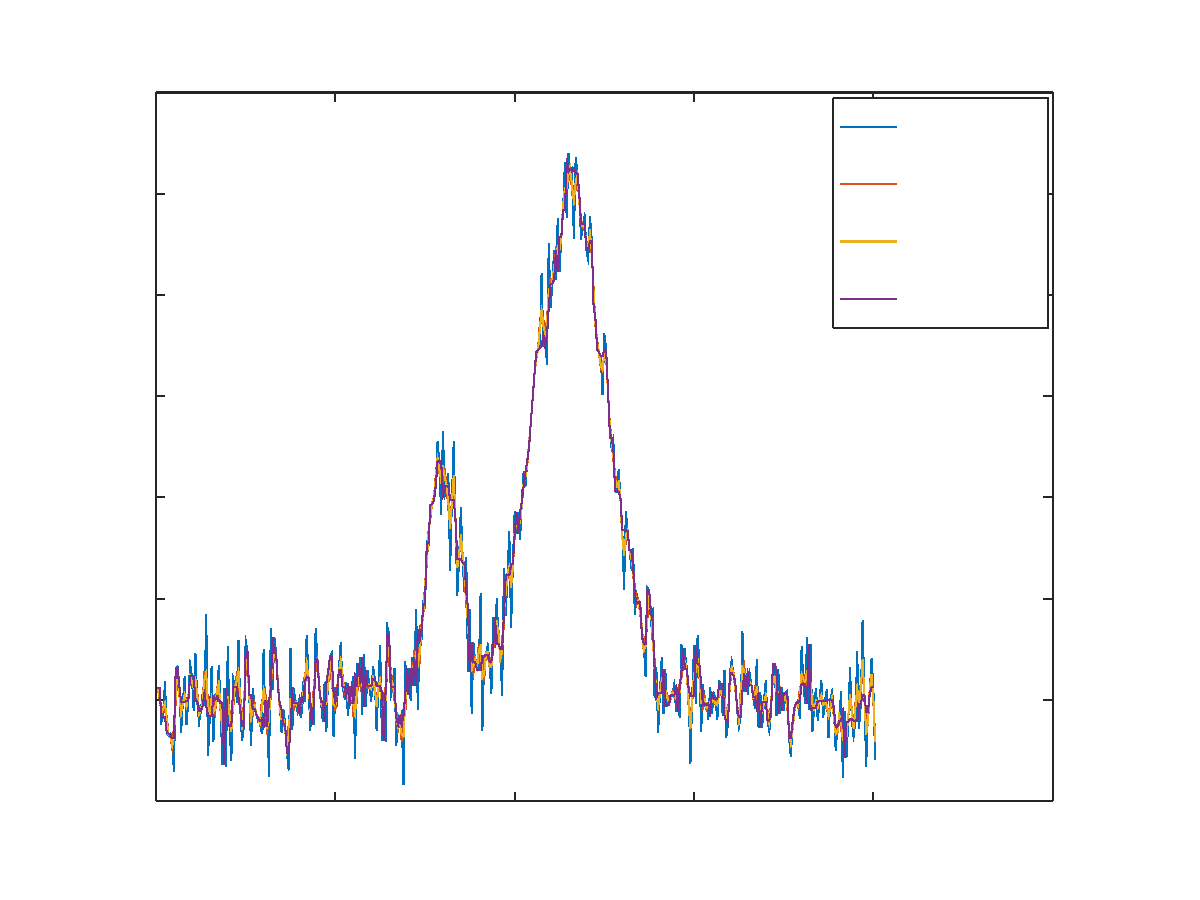
\includegraphics{low_pass_filters-inc}
\end{picture}%
\begin{picture}(576,432)(0,0)
\fontsize{12}{0}
\selectfont\put(74.88,42.5188){\makebox(0,0)[t]{\textcolor[rgb]{0.15,0.15,0.15}{{0}}}}
\fontsize{12}{0}
\selectfont\put(160.96,42.5188){\makebox(0,0)[t]{\textcolor[rgb]{0.15,0.15,0.15}{{100}}}}
\fontsize{12}{0}
\selectfont\put(247.04,42.5188){\makebox(0,0)[t]{\textcolor[rgb]{0.15,0.15,0.15}{{200}}}}
\fontsize{12}{0}
\selectfont\put(333.12,42.5188){\makebox(0,0)[t]{\textcolor[rgb]{0.15,0.15,0.15}{{300}}}}
\fontsize{12}{0}
\selectfont\put(419.2,42.5188){\makebox(0,0)[t]{\textcolor[rgb]{0.15,0.15,0.15}{{400}}}}
\fontsize{12}{0}
\selectfont\put(505.28,42.5188){\makebox(0,0)[t]{\textcolor[rgb]{0.15,0.15,0.15}{{500}}}}
\fontsize{12}{0}
\selectfont\put(69.8753,47.52){\makebox(0,0)[r]{\textcolor[rgb]{0.15,0.15,0.15}{{-1}}}}
\fontsize{12}{0}
\selectfont\put(69.8753,96.1029){\makebox(0,0)[r]{\textcolor[rgb]{0.15,0.15,0.15}{{0}}}}
\fontsize{12}{0}
\selectfont\put(69.8753,144.686){\makebox(0,0)[r]{\textcolor[rgb]{0.15,0.15,0.15}{{1}}}}
\fontsize{12}{0}
\selectfont\put(69.8753,193.269){\makebox(0,0)[r]{\textcolor[rgb]{0.15,0.15,0.15}{{2}}}}
\fontsize{12}{0}
\selectfont\put(69.8753,241.851){\makebox(0,0)[r]{\textcolor[rgb]{0.15,0.15,0.15}{{3}}}}
\fontsize{12}{0}
\selectfont\put(69.8753,290.434){\makebox(0,0)[r]{\textcolor[rgb]{0.15,0.15,0.15}{{4}}}}
\fontsize{12}{0}
\selectfont\put(69.8753,339.017){\makebox(0,0)[r]{\textcolor[rgb]{0.15,0.15,0.15}{{5}}}}
\fontsize{12}{0}
\selectfont\put(69.8753,387.6){\makebox(0,0)[r]{\textcolor[rgb]{0.15,0.15,0.15}{{6}}}}
\fontsize{12}{0}
\selectfont\put(290.08,397.6){\makebox(0,0)[b]{\textcolor[rgb]{0,0,0}{{Low-pass filters}}}}
\fontsize{12}{0}
\selectfont\put(433.703,371.177){\makebox(0,0)[l]{\textcolor[rgb]{0,0,0}{{$Y_{noise}$}}}}
\fontsize{12}{0}
\selectfont\put(433.703,343.628){\makebox(0,0)[l]{\textcolor[rgb]{0,0,0}{{$Y_{mean}$}}}}
\fontsize{12}{0}
\selectfont\put(433.703,316.08){\makebox(0,0)[l]{\textcolor[rgb]{0,0,0}{{$Y_{gaussian}$}}}}
\fontsize{12}{0}
\selectfont\put(433.703,288.531){\makebox(0,0)[l]{\textcolor[rgb]{0,0,0}{{$Y_{median}$}}}}
\end{picture}
}
 \caption{\label{fig:low_pass_filters}Low-pass filters.}
\end{figure}



\begin{figure}[htb]
\centering
\scalebox{0.75}{% Title: gl2ps_renderer figure
% Creator: GL2PS 1.3.9, (C) 1999-2015 C. Geuzaine
% For: Octave
% CreationDate: Mon Nov 27 09:16:12 2017
\setlength{\unitlength}{1pt}
\begin{picture}(0,0)
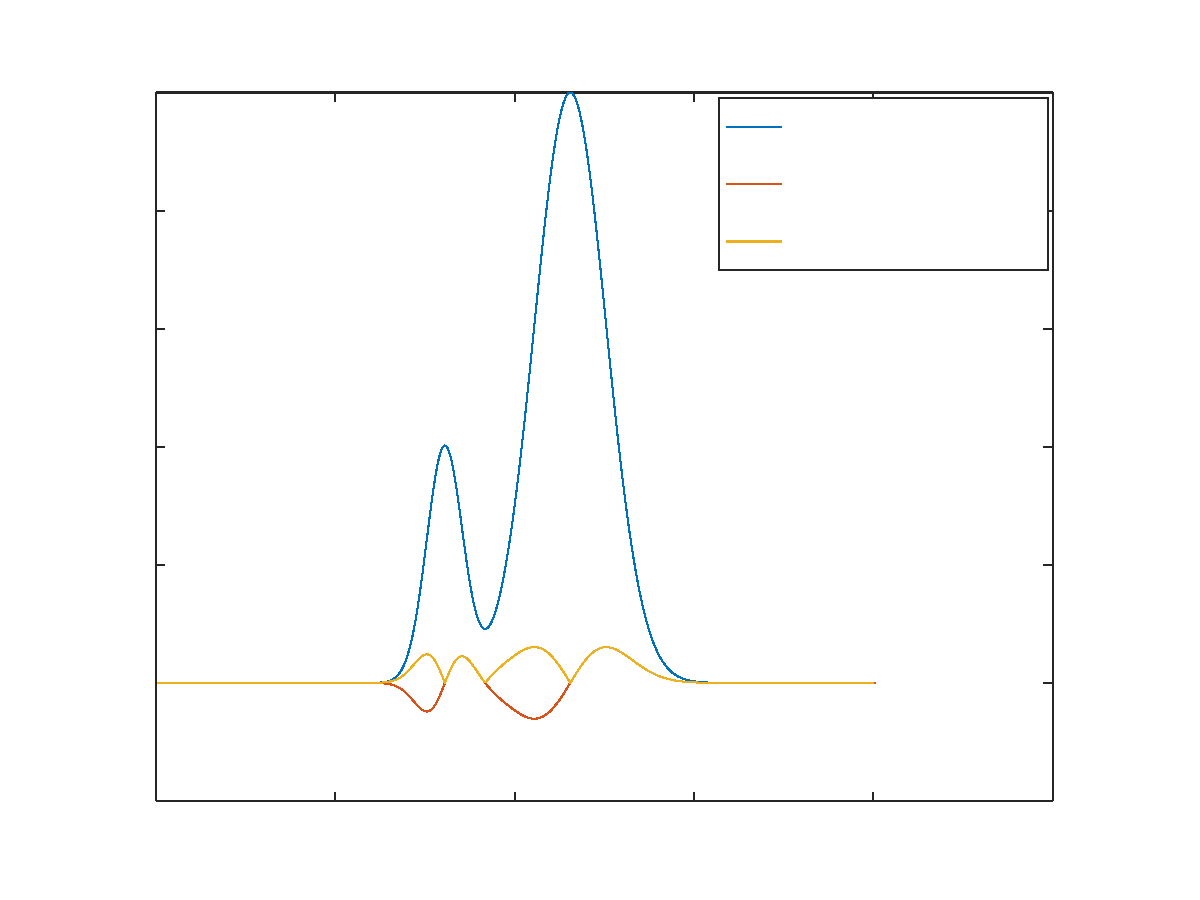
\includegraphics{high_pass_filters-inc}
\end{picture}%
\begin{picture}(576,432)(0,0)
\fontsize{12}{0}
\selectfont\put(74.88,42.5188){\makebox(0,0)[t]{\textcolor[rgb]{0.15,0.15,0.15}{{0}}}}
\fontsize{12}{0}
\selectfont\put(160.96,42.5188){\makebox(0,0)[t]{\textcolor[rgb]{0.15,0.15,0.15}{{100}}}}
\fontsize{12}{0}
\selectfont\put(247.04,42.5188){\makebox(0,0)[t]{\textcolor[rgb]{0.15,0.15,0.15}{{200}}}}
\fontsize{12}{0}
\selectfont\put(333.12,42.5188){\makebox(0,0)[t]{\textcolor[rgb]{0.15,0.15,0.15}{{300}}}}
\fontsize{12}{0}
\selectfont\put(419.2,42.5188){\makebox(0,0)[t]{\textcolor[rgb]{0.15,0.15,0.15}{{400}}}}
\fontsize{12}{0}
\selectfont\put(505.28,42.5188){\makebox(0,0)[t]{\textcolor[rgb]{0.15,0.15,0.15}{{500}}}}
\fontsize{12}{0}
\selectfont\put(69.8753,47.52){\makebox(0,0)[r]{\textcolor[rgb]{0.15,0.15,0.15}{{-1}}}}
\fontsize{12}{0}
\selectfont\put(69.8753,104.2){\makebox(0,0)[r]{\textcolor[rgb]{0.15,0.15,0.15}{{0}}}}
\fontsize{12}{0}
\selectfont\put(69.8753,160.88){\makebox(0,0)[r]{\textcolor[rgb]{0.15,0.15,0.15}{{1}}}}
\fontsize{12}{0}
\selectfont\put(69.8753,217.56){\makebox(0,0)[r]{\textcolor[rgb]{0.15,0.15,0.15}{{2}}}}
\fontsize{12}{0}
\selectfont\put(69.8753,274.24){\makebox(0,0)[r]{\textcolor[rgb]{0.15,0.15,0.15}{{3}}}}
\fontsize{12}{0}
\selectfont\put(69.8753,330.92){\makebox(0,0)[r]{\textcolor[rgb]{0.15,0.15,0.15}{{4}}}}
\fontsize{12}{0}
\selectfont\put(69.8753,387.6){\makebox(0,0)[r]{\textcolor[rgb]{0.15,0.15,0.15}{{5}}}}
\fontsize{12}{0}
\selectfont\put(290.08,397.6){\makebox(0,0)[b]{\textcolor[rgb]{0,0,0}{{High-pass filters}}}}
\fontsize{12}{0}
\selectfont\put(378.703,371.177){\makebox(0,0)[l]{\textcolor[rgb]{0,0,0}{{$Y$}}}}
\fontsize{12}{0}
\selectfont\put(378.703,343.628){\makebox(0,0)[l]{\textcolor[rgb]{0,0,0}{{$Y_derivative$}}}}
\fontsize{12}{0}
\selectfont\put(378.703,316.08){\makebox(0,0)[l]{\textcolor[rgb]{0,0,0}{{$Y_{gradient magnitude}$}}}}
\end{picture}
}
 \caption{\label{fig:high_pass_filters}High-pass filters.}
\end{figure}

\begin{lstlisting}
clear
close all

y = load("../data/y.mat");
y_noise = load("../data/y_noise.mat");

mean_filter = load("mean_filter.mat");
gaussian_filter = load("gaussian_filter.mat");
derivative_filter = load("derivative_filter.mat");
gradient_magnitude = load("gradient_magnitude.mat");
median_filter = load("median_filter.mat");


x=[1:size(y,2)]

figure;plot(x,y_noise,x,mean_filter,x,gaussian_filter,x,median_filter)
legend('$Y_{noise}$','$Y_{mean}$', '$Y_{gaussian}$', '$Y_{median}$')
title('Low-pass filters')
%print -dpdflatex -F:12 -color low_pass_filters.tex

figure;plot(x,y,x,derivative_filter,x,gradient_magnitude)
legend('$Y$','$Y_derivative$', '$Y_{gradient magnitude}$')
title('High-pass filters')
%print -dpdflatex -F:12 -color high_pass_filters.tex
\end{lstlisting}
%\item $NCC_y_y_quadriple =  99.751$
%\item $NCC_y_y_negative = -99.751$
%\item $NCC_y_y_noise =  96.845$


%
%
%
%
%
%
%For this task, you are given two C++ files:
%\begin{enumerate}
%  \item \verb+include/Utils.h+, a header file with the declarations of some functions.
%  \item \verb+src/TestVector.cpp+, a test program to try the vector class.
%\end{enumerate}
%
%Modify \verb+include/Utils.h+ to convert every function as a template function. 
%To implement every function, you need to write the code directly in the header. 
%In \verb+src/TestVector.cpp+, test every template function with different data types.
%
%
%\section*{Task 3: Create your own template class}
%
%This time, you have to create your own files and modify CMakeLists.txt. 
%We propose to create a template class to handle square matrices, e.g. n-by-n matrices. 
%The class should contain:
%\begin{itemize}
%\item a default constructor, 
%\item a copy constructor, 
%\item a copy operator, 
%\item \verb+operator<<+, 
%\item \verb+operator>>+,
%\item \verb+unsigned int m_size+ (default: 4) the number of rows 
%\item \verb+unsigned int getSize() const+
%\item \verb+void setSize(unsigned int)+
%\item \verb+T& get(unsigned int i, unsigned int j) const+
%\item \verb+void set(unsigned int i, unsigned int j, const T& aValue)+
%\item \verb+void setIdentity()+
%\end{itemize}
%Each method should be tested and validated in a test program. 
%Do not wait until the end to test your code. 
%A good programming strategy is to test a function just after it has been implemented. 


\section*{Task 6: Assignment 2}

Adapt the code to handle 2-D signals  (images) 
 Assignment~2, you have to do tin your assignments.he same in 2-D with images. 
 
 In 1-D, we had one loop for all the elements of the signal, and one loop for all the elements of the kernel. 
 In 2-D, we will have four nested loops:
 \begin{enumerate}
 \item One for the rows of the image;
 \item One for the columns of the image;
 \item One for the rows of the kernel;
 \item One for the columns of the kernel.
 \end{enumerate}
 
 
 
$m$ is the input image, and $g$ is the kernel (sliding window). 
$m$  has a width of $W_m$ and height of $H_m$,
$g$  has a width of $W_g$ and height of $H_g$.
$m'$ is the result of the convolution of $m$ by $g$: %$(m'(i) = (m * g)(i)$.

$$
m'(i,j) = (m * g)(i,j) = \sum^{l < H_g}_{l=0}\sum^{k < W_g}_{k=0} m(i - W_g \setminus 2 + k, j - H_g \setminus + l) \times g(k,l)
$$
with $i$ the pixel index along the X-axis, and $j$ the pixel index along the Y-axis.
 
\end{document}
